\documentclass{article}
\usepackage[utf8]{inputenc}
\usepackage[english,serbian]{babel}
\usepackage{amsmath}
\usepackage{circuitikz}
    \usetikzlibrary{arrows}
\usepackage{enumitem}
\usepackage{graphicx}
\usepackage{float}
\usepackage{listings}
\usepackage{pdfpages}
\usepackage{siunitx}
\usepackage[a4paper,left=1in,top=1in,right=1in,bottom=1in,nohead]{geometry}
\usepackage{xcolor}
\setlist[enumerate,1]{% (
leftmargin=*, itemsep=12pt, label={\textbf{\arabic*.}}}

\lstnewenvironment{spiceoutput}[1][]{
    \lstset{escapeinside={(*@}{@*)},
    framesep=5pt,
    basicstyle=\normalsize\ttfamily,
    showstringspaces=false,
    keywordstyle=\itshape\color{blue},
    stringstyle=\color{maroon},
    commentstyle=\color{black},
    rulecolor=\color{black},
    xleftmargin=0pt,
    xrightmargin=0pt,
    aboveskip=\medskipamount,
    belowskip=\medskipamount,
   backgroundcolor=\color{white}, #1
}}{}

\title{Treći domaći zadatak iz Osnova elektronike}
\author{Luka Simić, 19/0368}
\date{}

\begin{document}

    \begin{titlepage}
        \maketitle
    \end{titlepage}

    \section{Postavka}
        \begin{enumerate}[itemsep=\baselineskip]
            \item Na slici \ref{Postavka}, prikazan je pojačavač sa zajedničkim emitorom sa strujnim izvorom za podešavanje mirne radne tačke.
    
            \textbf{a)} Odrediti vrednosti svih otpornika tako da jednosmerni napon kolektora tranzistora $Q_2$ bude 8V, jednosmerni napon emitora tranzistora $Q_2$ bude 4V, a jednosmerna struja $I_{C_2}$ bude 1mA. Rezultat verifikovati simulacijom, a jednosmerne potencijale čvorova i struje tranzistora prikazati slikom dobijenom nakon simulacionog određivanja mirne radne tačke.
    
            \textbf{b)} Odrediti parametre za mali signal $g_m$ i $r_\pi$. Verifikovati rezultat uvidom u izlazni fajl simulatora čiji relevantni deo treba ubaciti u izveštaj.
    
            \textbf{c)} Odrediti vrednosti svih kondenzatora u kolu tako da moduo njihove impedanse na učestanosti od značaja bude bar 100 puta manji od otpornosti u kolu.
    
            \textbf{d)} Odrediti pojačanje za mali signal, ulaznu i izlaznu otpornost. Rezultat verifikovati simulacijom, a relevantne grafike koji dokazuju rezultate ubaciti u izveštaj.
        \end{enumerate}
        \begin{figure}[H]
            \centering
            \begin{circuitikz}[american voltages]
                \draw [-latex] (7, 7) -- (8, 7) node[below] {$V_{CC}$};
                \draw
                % Ground to BJT
                (0, 0) to node[ground]{} (0, 1)
                to [vsourcesin, l=$v_u$] (0, 4)
                to [capacitor, l=$C_1$] (3, 4)
                to [short] (4, 4)
                % Vcc
                (0, 7) to [short] (7, 7)
                % R3 to mirror
                (1, 7) to [R, l=$R_3$, *-] (1, 5)
                to [short, -*] (1, 2)
                to [short] (1.8, 2)
                to [short, -*] (1.8, 1.25)
                to [short] (4, 1.25)
                % R2 to C1
                (3, 7) to [R, l=$R_2$, *-] (3, 5)
                to [short, -*] (3, 4)
                % R1 to between transistors
                (4.84, 7) to [R, l=$R_1$, *-] (4.84, 4.8)
                to [short, *-*] (6, 4.8)
                to [R, l=$R_4$] (6, 3)
                to [short, *-*] (4.84, 3)
                % Between transistors
                (4.84, 3.21) to [short] (4.84, 2.01)
                % C2 to ground
                (6, 4.8) to [capacitor, l=$C_2$] (8, 4.8)
                to [short, -*, l_=$v_i$] (8, 4.8)
                to [R, l=$R_p$] (8, 2)
                to [short] (8, 0.5)
                % C3 to ground
                (6, 3) to [capacitor, l=$C_3$] (6, 1)
                to [short, -*] (6, 0.5)
                % GND
                (0, 0.5) to [short, -*] (1, 0.5)
                to [short, -*] (4.84, 0.5)
                to [short] (8, 0.5)
                % Transistors
                (1, 2) to node[npn, anchor=C, xscale=-1]{} (1, 2)
                (4, 1.25) to node[npn, anchor=B]{} (4, 1.25)
                (4, 4) to node[npn, anchor=B]{} (4, 4)
                (5.25, 1.55) node[below]{$Q_1$}
                (5.25, 4.3) node[below]{$Q_2$}
                (0.5, 1.55) node[below]{$Q_4$}
                ;
            \end{circuitikz}
            \caption{Pojačavač sa zajedničkim emitorom sa strujnim izvorom za podešavanje mirne radne tačke}
            \label{Postavka}
        \end{figure}

    \section{Rešenje}
        \subsection{Prvi deo}
            Pošto u prva tri dela zadatka možemo raditi samo u DC režimu, možemo raditi sa ekvivalentnim kolom za DC režim sa slike \ref{DC1}.
            \begin{figure}[H]
                \centering
                \begin{circuitikz}[american voltages]
                    \draw [-latex] (7, 7) -- (8, 7) node[below] {$V_{CC}$};
                    \draw [-latex] (4.84, 4.8) -- (4.84, 4.5) node[left] {$I_{C_2}$};
                    \draw
                    % Ground
                    (1, 0) to node[ground]{} (1, 1)
                    % Vcc
                    (1, 7) to [short] (7, 7)
                    % R3 to mirror
                    (1, 7) to [R, l=$R_3$, i=$I_{R_3}$] (1, 5)
                    to [short, -*] (1, 2)
                    to [short] (1.8, 2)
                    to [short, -*] (1.8, 1.25)
                    to [short] (4, 1.25)
                    % R2 to BJT
                    (3, 7) to [R, l=$R_2$] (3, 5)
                    to [short] (3, 4)
                    to [short, i=$I_{B_2}$] (4, 4)
                    % R1 to between transistors
                    (4.84, 7) to [R, l=$R_1$, i=$I_{R_1}$] (4.84, 4.8)
                    to [short, *-] (6, 4.8)
                    to [R, l=$R_4$, i=$I_{R_4}$] (6, 3)
                    to [short, -*] (4.84, 3)
                    % Between transistors
                    (4.84, 3.21) to [short, i_=$I_{E_2}$] (4.84, 3)
                    to [short, i=$I_{C_1}$] (4.84, 2.01)
                    % GND
                    (1, 0.5) to [short, *-*] (4.84, 0.5)
                    to [short] (8, 0.5)
                    % Transistors
                    (1, 2) to node[npn, anchor=C, xscale=-1]{} (1, 2)
                    (4, 1.25) to node[npn, anchor=B]{} (4, 1.25)
                    (4, 4) to node[npn, anchor=B]{} (4, 4)
                    (5.25, 1.55) node[below]{$Q_1$}
                    (5.25, 4.3) node[below]{$Q_2$}
                    (0.5, 1.55) node[below]{$Q_4$}
                    ;
                \end{circuitikz}
                \caption{Ekvivalentno kolo za DC režim}
                \label{DC1}
            \end{figure}
            Po propozicijama zadatka imamo napon kolektora i emitora tranzistora $Q_2$, kao i struju kolektora tog tranzistora.
            \begin{equation}
                \label{VC2}
                V_{C_2} = 8V
            \end{equation}
            \begin{equation}
                \label{VE2}
                V_{E_2} = 4V
            \end{equation}
            \begin{equation}
                \label{IC2}
                I_{C_2} = 1mA
            \end{equation}
            Na osnovu \eqref{VC2} i \eqref{VE2} možemo izraziti struju kroz otpornike $R_4$ i $R_1$.
            \begin{equation}
                \label{IR4}
                I_{R_4} = \frac{V_{C_2} - V_{E_2}}{R_4} = \frac{8V - 4V}{4k\Omega} = 1mA
            \end{equation}
            \begin{equation}
                \label{IR1}
                I_{R_1} = \frac{V_{CC} - V_{C_2}}{R_1}
            \end{equation}
            Pošto imamo $V_{BE} = 0.7V$ kao parametar tehnologije možemo izračunati i napon baze $Q_2$.
            \begin{equation}
                \label{VB2}
                V_{B_2} = V_{E_2} + V_{BE} = 4.7V
            \end{equation}
            Pa iz \eqref{VB2} možemo izraziti i struju baze $Q_2$.
            \begin{equation}
                \label{IB2}
                I_{B_2} = \frac{V_{CC} - V_{B_2}}{R_2}
            \end{equation}
            Možemo takođe primetiti da se tranzistori $Q_1$ i $Q_4$ nalaze u strujnom ogledalu i stoga su im sve struje iste.
            \begin{equation}
                \label{IC1}
                I_{C_1} = I_{C_4}
            \end{equation}
            \begin{equation}
                \label{IB1}
                I_{B_1} = I_{B_4}
            \end{equation}
            Takođe, možemo primetiti da je napon baza $Q_1$ i $Q_4$, kao i napon kolektora $Q_4$, jednak naponu između emitora i baze tranzistora $Q_4$, jer je emitor $Q_4$ uzemljen.
            \begin{equation}
                \label{VC4}
                V_{B_1} = V_{B_4} = V_{C_4} = V_{BE}
            \end{equation}
            Iz \eqref{VC4} možemo izraziti struju kroz otpornik $R_3$.
            \begin{equation}
                \label{IR3}
                I_{R_3} = \frac{V_{CC} - V_{C_4}}{R_3} = \frac{V_{CC} - V_{BE}}{R_3}
            \end{equation}
            Dalje, iz jednačina za struje tranzistora $Q_2$ možemo dobiti vrednosti struja $I_{B_2}$ i $I_{E_2}$.
            \begin{equation}
                \label{IB22}
                I_{B_2} = \frac{I_{C_2}}{\beta} = \frac{1mA}{100} = 10\mu A
            \end{equation}
            \begin{equation}
                \label{IE2}
                I_{E_2} = (\beta + 1) I_{B_2} = \frac{101}{100} 1mA = 1.01mA
            \end{equation}
            Takođe, iz jednačina za struje tranzistora $Q_4$, \eqref{IB1} i \eqref{IC1} možemo izraziti struje baza tranzistora $Q_1$ i $Q_4$.
            \begin{equation}
                \label{IB12}
                I_{B_1} = I_{B_4} = \frac{I_{C_4}}{\beta} = \frac{I_{C_1}}{100}
            \end{equation}
            Iz \eqref{IC2}, \eqref{IR4} i Kirhofovog zakona za struje u čvoru iznad kolektora $Q_2$ dobijamo vrednost struje $I_{R_1}$.
            \begin{equation}
                \label{IR12}
                I_{R_1} = I_{C_2} + I_{R_4} = 2mA
            \end{equation}
            Iz \eqref{IE2}, \eqref{IR4} i Kirhofovog zakona za struje u čvoru ispod emitera $Q_2$ dobijamo vrednost struje $I_{C_1}$.
            \begin{equation}
                \label{IC12}
                I_{C_1} = I_{E_2} + I_{R_4} = 1.01mA + 1mA = 2.01mA
            \end{equation}
            Iz \eqref{IC1}, \eqref{IC12}, \eqref{IB12} i Kirhofovog zakona za struje u čvoru iznad kolektora $Q_4$ dobijamo vrednost struje $I_{R_3}$.
            \begin{equation}
                \label{IR31}
                I_{R_3} = I_{B_1} + I_{B_4} + I_{C_4} = I_{C_1} + \frac{I_{C_1}}{100} + \frac{I_{C_1}}{100} = \frac{102}{100} 2.01mA = 2.0502mA
            \end{equation}
            Iz \eqref{VC2}, \eqref{IR1} i \eqref{IR12} dobijamo otpornost otpornika $R_1$.
            $$R_1 = \frac{V_{CC} - V_{C_2}}{I_{R_1}} = \frac{12V - 8V}{2mA} = \frac{4V}{2mA}$$
            $$\boxed{R_1 = 2k\Omega}$$
            Iz \eqref{VB2}, \eqref{IB2} i \eqref{IB22} dobijamo otpornost otpornika $R_2$.
            $$R_2 = \frac{V_{CC} - V_{B_2}}{I_{B_2}} = \frac{12V - 4.7V}{10\mu A} = \frac{7.3V}{10\mu A}$$
            $$\boxed{R_2 = 730k\Omega}$$
            Iz \eqref{IR3}, \eqref{IR31} dobijamo otpornost otpornika $R_3$.
            $$R_3 = \frac{V_{CC} - V_{BE}}{I_{R_3}} = \frac{12V - 0.7V}{2.0502mA} = \frac{11.3V}{2.0502mA}$$
            $$\boxed{R_3 \approx 5.512k\Omega}$$
            Simulacijom u \textit{PSpice}-u sa izračunatim otpornostima dobijamo vrednosti DC napona i struja kao sa slike \ref{Prvi} koji su približno jednaki vrednostima u postavci zadatka (sa greškom manjom od 1\%).
            \begin{figure}[H]
                \centering
                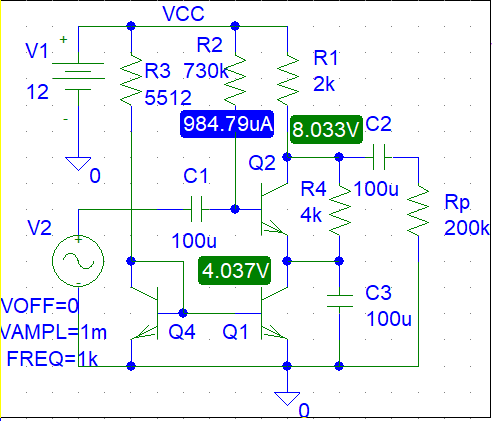
\includegraphics{Prvi.png}
                \caption{Rezultat simulacije kola u \textit{PSpice}-u za prvi deo zadatka. Prikazani su naponi $V_{C_2}$, $V_{E_2}$ i struja $I_{C_2}$}
                \label{Prvi}
            \end{figure}

        \subsection{Drugi deo}
            Iz \eqref{IC1} i \eqref{IC12} dobijamo parametre za mali signal tranzistora $Q_1$ i $Q_4$.
            $$g_{m_1} = g_{m_4} = \frac{I_{C_1}}{V_T} = \frac{2.01mA}{25mV}$$
            $$\boxed{g_{m_1} = g_{m_4} = 80.4mS}$$
            $$r_{\pi_1} = r_{\pi_4} = \frac{\beta}{g_{m_1}} = \frac{100}{80.4mS}$$
            $$\boxed{r_{\pi_1} = r_{\pi_4} = 1.24378k\Omega}$$
            Iz \eqref{IC2} dobijamo parametre za mali signal tranzistora $Q_2$.
            $$g_{m_2} = \frac{I_{C_2}}{V_T} = \frac{1mA}{25mV}$$
            $$\boxed{g_{m_2} = 40mS}$$
            $$r_{\pi_2} = \frac{\beta}{g_{m_2}} = \frac{100}{40mS}$$
            $$\boxed{r_{\pi_2} = 2.5k\Omega}$$
            Možemo videti da se i \textit{PSpice} simulacijom dobijaju slične vrednosti za parametre za mali signal na figuri \ref{Drugi}.

            \begin{figure}[H]
                \centering
                \begin{spiceoutput}
**** BIPOLAR JUNCTION TRANSISTORS


NAME         Q_Q1        Q_Q2        Q_Q4     
MODEL        QbreakN     QbreakN     QbreakN  
IB           1.99E-05    9.85E-06    1.99E-05 
IC           1.99E-03    9.85E-04    1.99E-03 
VBE          7.92E-01    7.74E-01    7.92E-01 
VBC         -3.25E+00   -3.22E+00    0.00E+00 
VCE          4.04E+00    4.00E+00    7.92E-01 
BETADC       1.00E+02    1.00E+02    1.00E+02 
(*@\textcolor{red}{GM}@*)           (*@\textcolor{red}{7.71E-02}@*)      (*@\textcolor{red}{3.81E-02}@*)     (*@\textcolor{red}{7.71E-02}@*) 
(*@\textcolor{red}{RPI}@*)          (*@\textcolor{red}{1.30E+03}@*)      (*@\textcolor{red}{2.63E+03}@*)     (*@\textcolor{red}{1.30E+03}@*) 
RX           0.00E+00    0.00E+00    0.00E+00 
RO           1.00E+12    1.00E+12    9.96E+11 
CBE          0.00E+00    0.00E+00    0.00E+00 
CBC          0.00E+00    0.00E+00    0.00E+00 
CJS          0.00E+00    0.00E+00    0.00E+00 
BETAAC       1.00E+02    1.00E+02    1.00E+02 
CBX/CBX2     0.00E+00    0.00E+00    0.00E+00 
FT/FT2       1.23E+18    6.06E+17    1.23E+18 
                \end{spiceoutput}
                \caption{Parametri tranzistora za mali signal iz ispisa \textit{PSpice} simulacije. Crvenom bojom označene su relevantne linije koje dokazuju izračunate rezultate.}
                \label{Drugi}
            \end{figure}

        \subsection{Treći deo}
            Učestanost generatora $v_u$ se može izračunati na osnovu njene frekvencije.
            \begin{equation}
                \label{omega}
                \omega = 2\pi f = 2\pi \cdot 1kHz = 6283.18530 \frac{rad}{s}
            \end{equation}
            Pošto nam je najmanji otpornik u kolu $R_{min} = R_1 = 2k\Omega$ dobijamo kapacitivnost kondenzatora modula impedanse 100 puta manjeg od najmanje otpornosti.
            $$\frac{R_{min}}{100} = \left| \frac{-j}{\omega C} \right| = \frac{1}{\omega C}$$
            $$C = \frac{100}{\omega R_{min}} = \frac{100}{6283.18530 \frac{rad}{s} \cdot 2k\Omega}$$
            $$\boxed{C = 7.9577\mu F}$$
            U daljim simulacijama biće usvojena aproksimacija $C \approx 100\mu F$.

        \subsection{Četvrti deo}
            Kako bismo računski dobili rezultat možemo raditi sa ekvivalentnim kolom za male signale kao na slici \ref{AC1}. Kako se strujno ogledalo može ekvivalentirati nezavisnim strujnim generatorom u DC režimu, može se u potpunosti isključiti iz kola za male signale.
            \begin{figure}[H]
                \centering
                \begin{circuitikz}[american voltages]
                    \draw
                    % Ground
                    (0, 0) to node[ground]{} (0, 1)
                    (0, 0.5) to [short, *-] (5, 0.5)
                    % Generator to R2
                    (0, 1) to [vsourcesin, l=$v_u$] (0, 3)
                    to [short, -*, i=$i_u$] (1, 3)
                    to [R, l=$R_2$] (1, 1)
                    to [short, -*] (1, 0.5)
                    % R2 to emitter
                    (1, 3) to [short, i=$i_b$] (2, 3)
                    to [R, l=$r_{\pi_{2}}$] (2, 1)
                    to [short, -*] (3, 1)
                    to [short, -*] (3, 0.5)
                    % Emitter to ground
                    (3, 1) to [short] (4, 1)
                    to [american controlled current source, l=$\beta i_b$, invert] (4, 3)
                    to [short, -*, l=$v_i$] (5, 3)
                    to [R, l=$R_1 || R_4 || R_p$, i<=$\beta i_b$] (5, 0.5)
                    ;
                \end{circuitikz}
                \caption{Ekvivalentno kolo za male signale}
                \label{AC1}
            \end{figure}
            Struja baze jednaka je struji kroz otpornik $r_{\pi_2}$.
            \begin{equation}
                \label{ib}
                i_b = \frac{v_u}{r_{\pi_2}}
            \end{equation}
            Izlazni napon $v_i$ je stoga jednak padu napona na paralelnoj vezi otpornika $R_1$, $R_4$ i $R_p$, pa zavisnost $v_u$ od $v_i$ možemo da dobijemo iz \eqref{ib}.
            \begin{equation}
                \label{vi}
                v_i = -\beta i_b(R_1 || R_4 || R_p) = -\beta \frac{v_u}{r_{\pi_2}}(R_1 || R_4 || R_p)
            \end{equation}
            Iz \eqref{vi} dobijamo da nam je naponsko pojačanje za male signale:
            $$A_v = -\beta \frac{R_1 || R_4 || R_p}{r_{\pi_2}} = -100 \frac{2k\Omega || 4k\Omega || 200k\Omega}{2.5k\Omega}$$
            $$\boxed{A_v = -52.9801}$$
            Ulaznu struju možemo izračunati kao struju kroz paralelnu vezu otpornika $R_2$ i $r_{\pi_2}$ do uzemljenja.
            \begin{equation}
                \label{iu}
                i_u = \frac{v_u}{R_2 || r_{\pi_2}}
            \end{equation}
            Izlaznu struju možemo izračunati kao struju kroz otpornik $R_p$ do uzemljenja.
            \begin{equation}
                \label{ii}
                i_i = \frac{v_i}{R_p}
            \end{equation}
            Iz \eqref{iu} i \eqref{ii} dobijamo da nam je strujno pojačanje za male signale:
            $$A_i = \frac{i_i}{i_u} = \frac{\frac{v_i}{R_p}}{\frac{v_u}{R_2 || r_{\pi_2}}} = \frac{-52.9801 v_u (730k\Omega || 2.5k\Omega)}{v_u \cdot 200k\Omega}$$
            $$\boxed{A_i \approx -0.66}$$
            Ove rezultate potrvrđuje poklapanje grafika ulaznog i izlaznog napona (odnosno struje) \textit{PSpice} simulacije na slikama \ref{Naponsko} i \ref{Strujno} kada se ulazna strana pomnoži sa izračunatim pojačanjem.
            \begin{figure}[H]
                \centering
                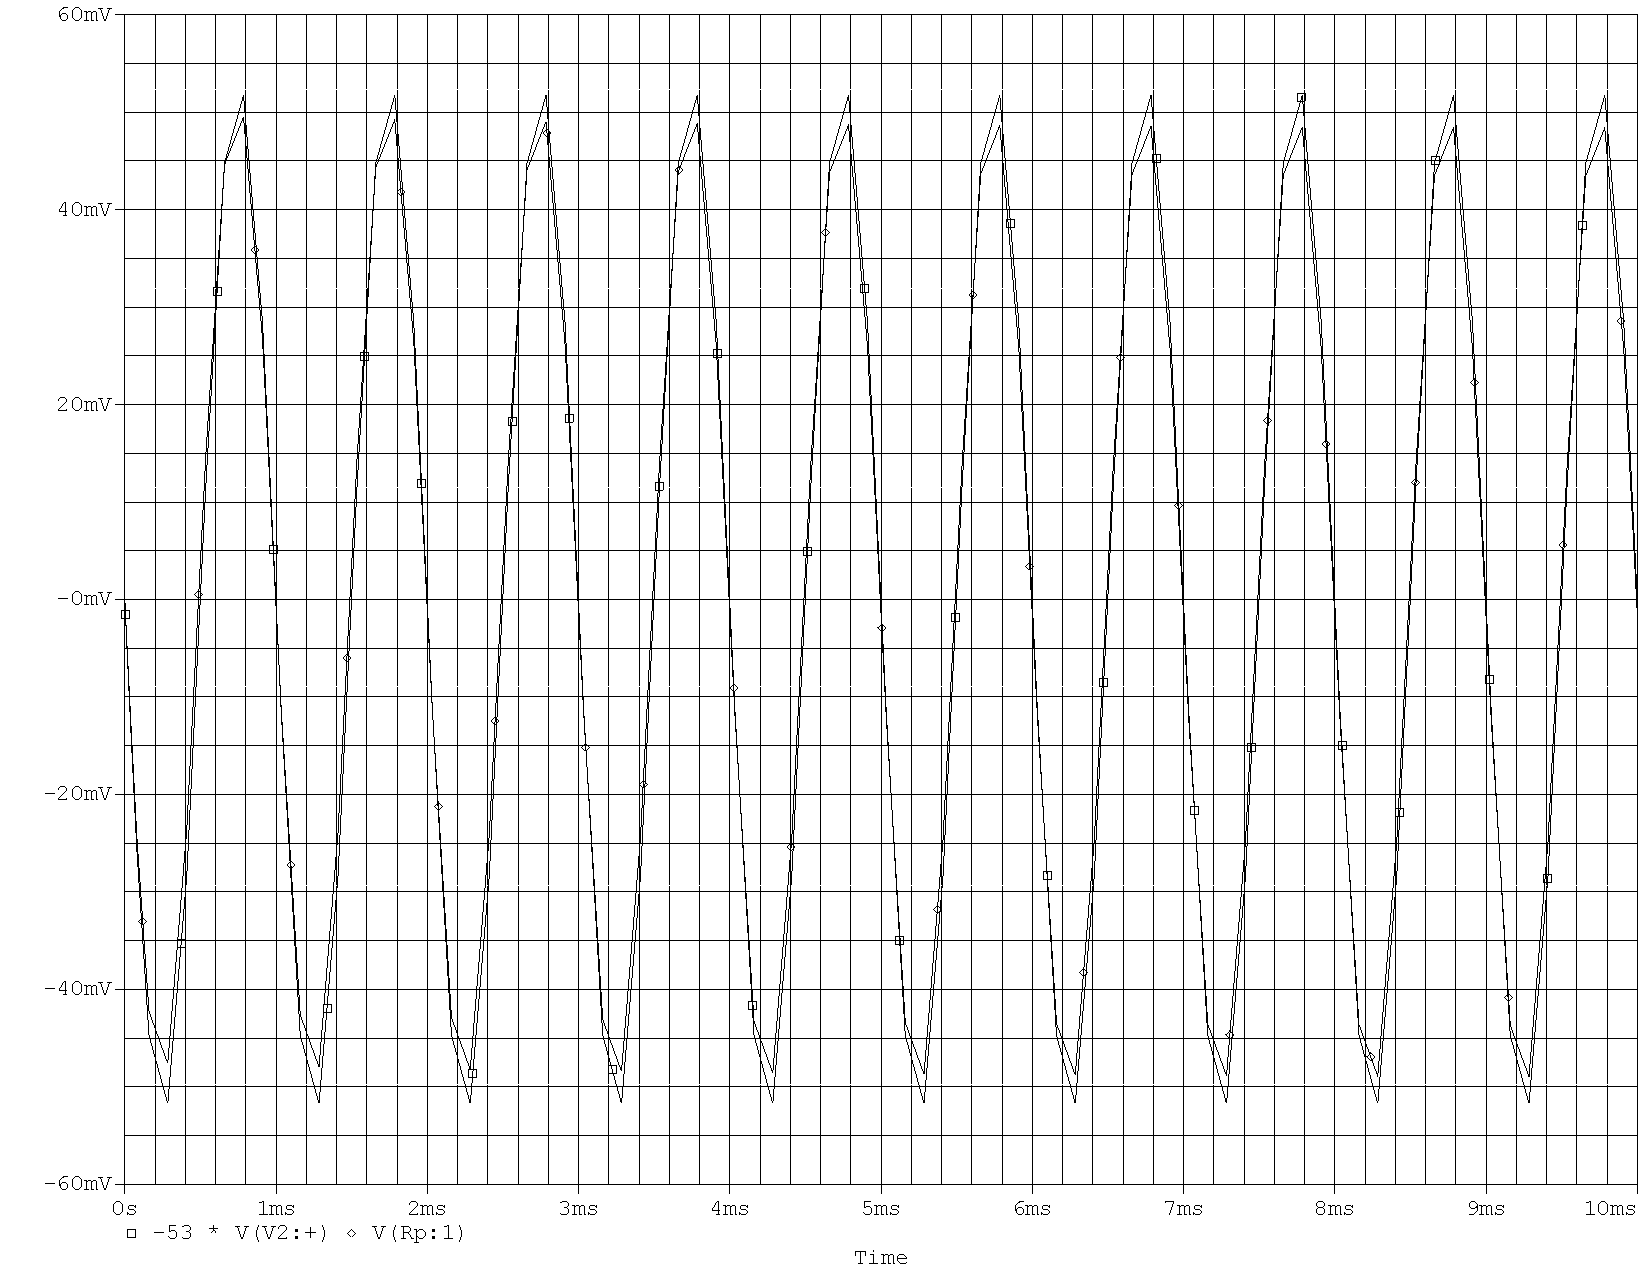
\includegraphics[width=\textwidth,height=\textheight,keepaspectratio]{Naponsko.pdf}
                \caption{Grafik za verifikaciju naponskog pojačanja}
                \label{Naponsko}
            \end{figure}
            \begin{figure}[H]
                \centering
                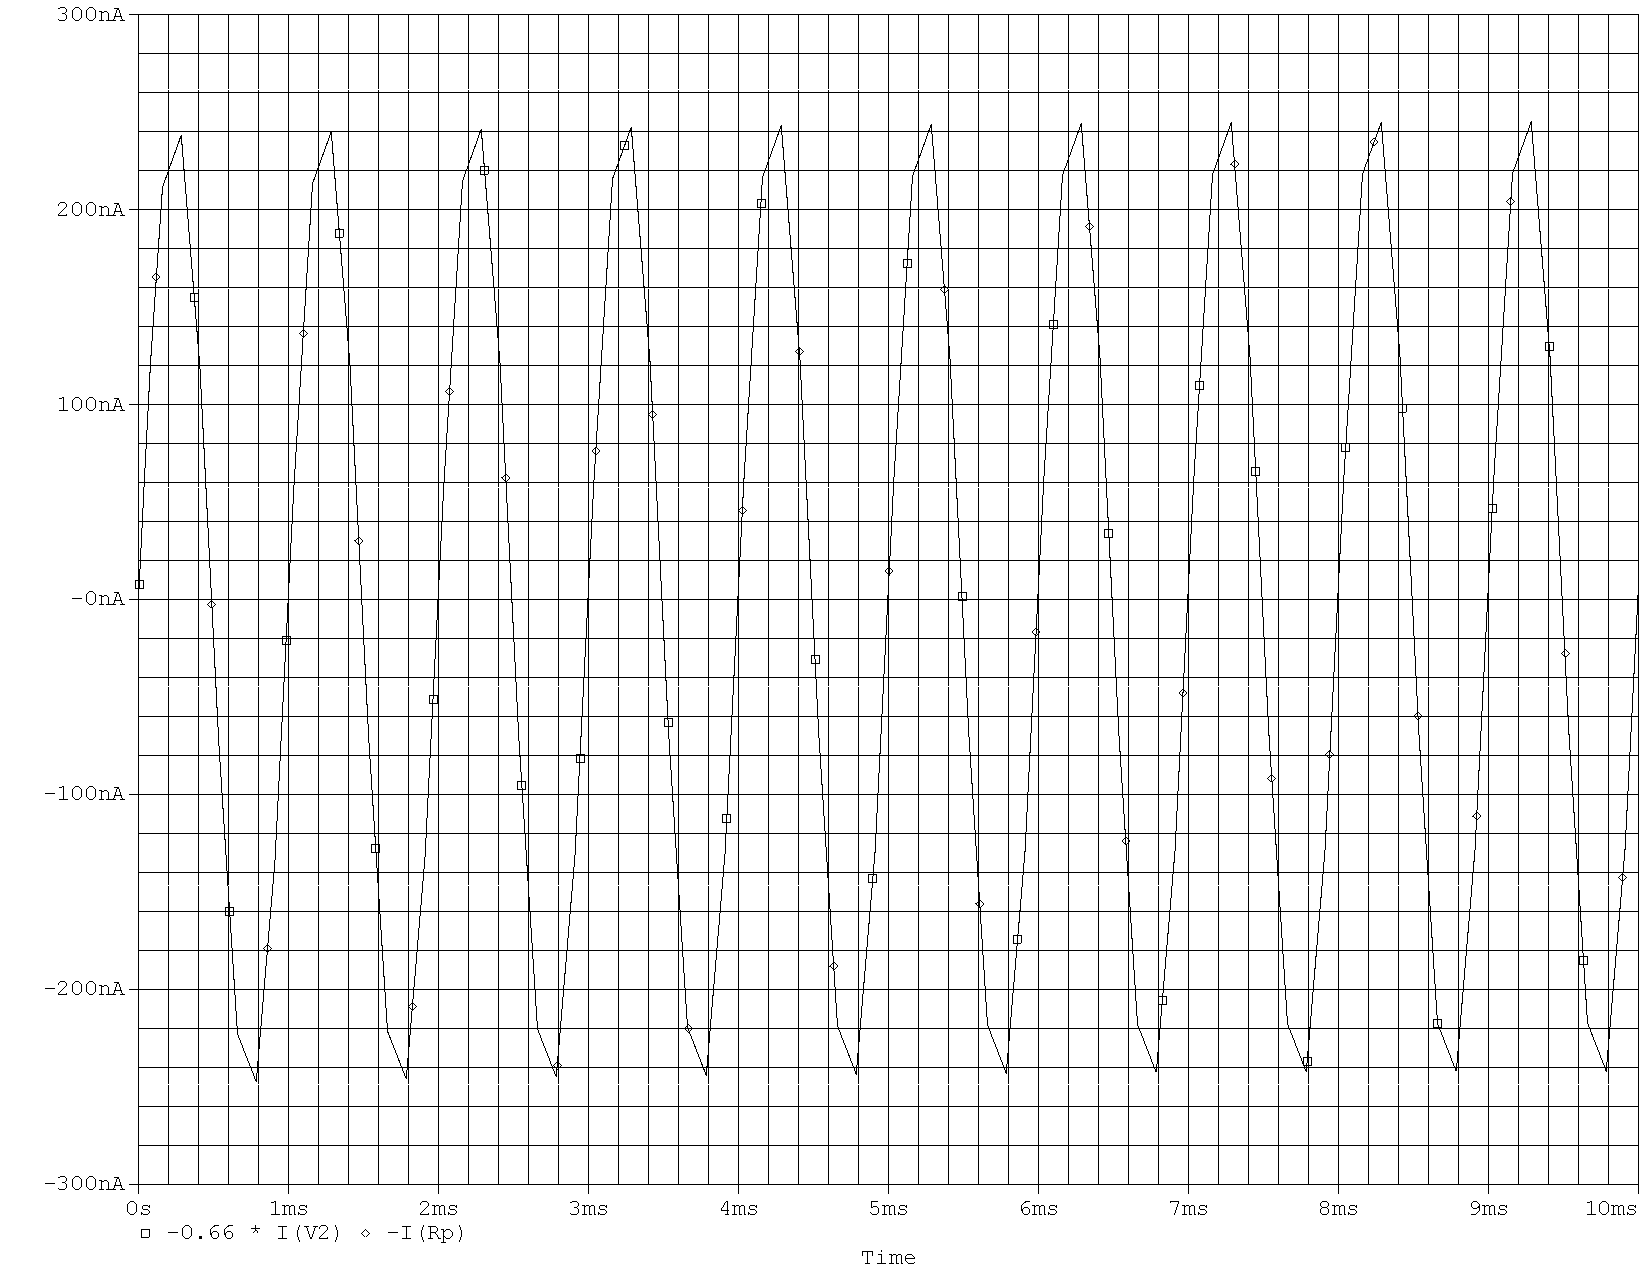
\includegraphics[width=\textwidth,height=\textheight,keepaspectratio]{Strujno.pdf}
                \caption{Grafik za verifikaciju strujnog pojačanja}
                \label{Strujno}
            \end{figure}
            Na osnovu \eqref{iu} takođe dobijamo ulaznu otpornost.
            $$r_u = R_2 || r_{\pi_2}$$
            $$\boxed{r_u \approx 2.5k\Omega}$$
            Kada otpornik $R_p$ zamenimo naponskim generatorom i ukinemo generator $v_u$, zavisni strujni generator nam postaje otvorena veza, pa je izlazna otpornost jednaka:
            $$r_i = R_1 || R_4 = 2k\Omega || 4k\Omega$$
            $$\boxed{r_i \approx 1.33k\Omega}$$
            Ove rezultate potrvrđuju grafici dobijeni \textit{PSpice} simulacijom nad kolom sa slike \ref{CetvrtiKolo} sa slika \ref{Izlazna} i \ref{Ulazna}. Kako količnik napona i struje test generatora nema smisla kada je struja test generatora nula, simulacija nije rađena na dužem vremenu kako se ne bi poklopila sa takvim tačkama.
            \begin{figure}[H]
                \centering
                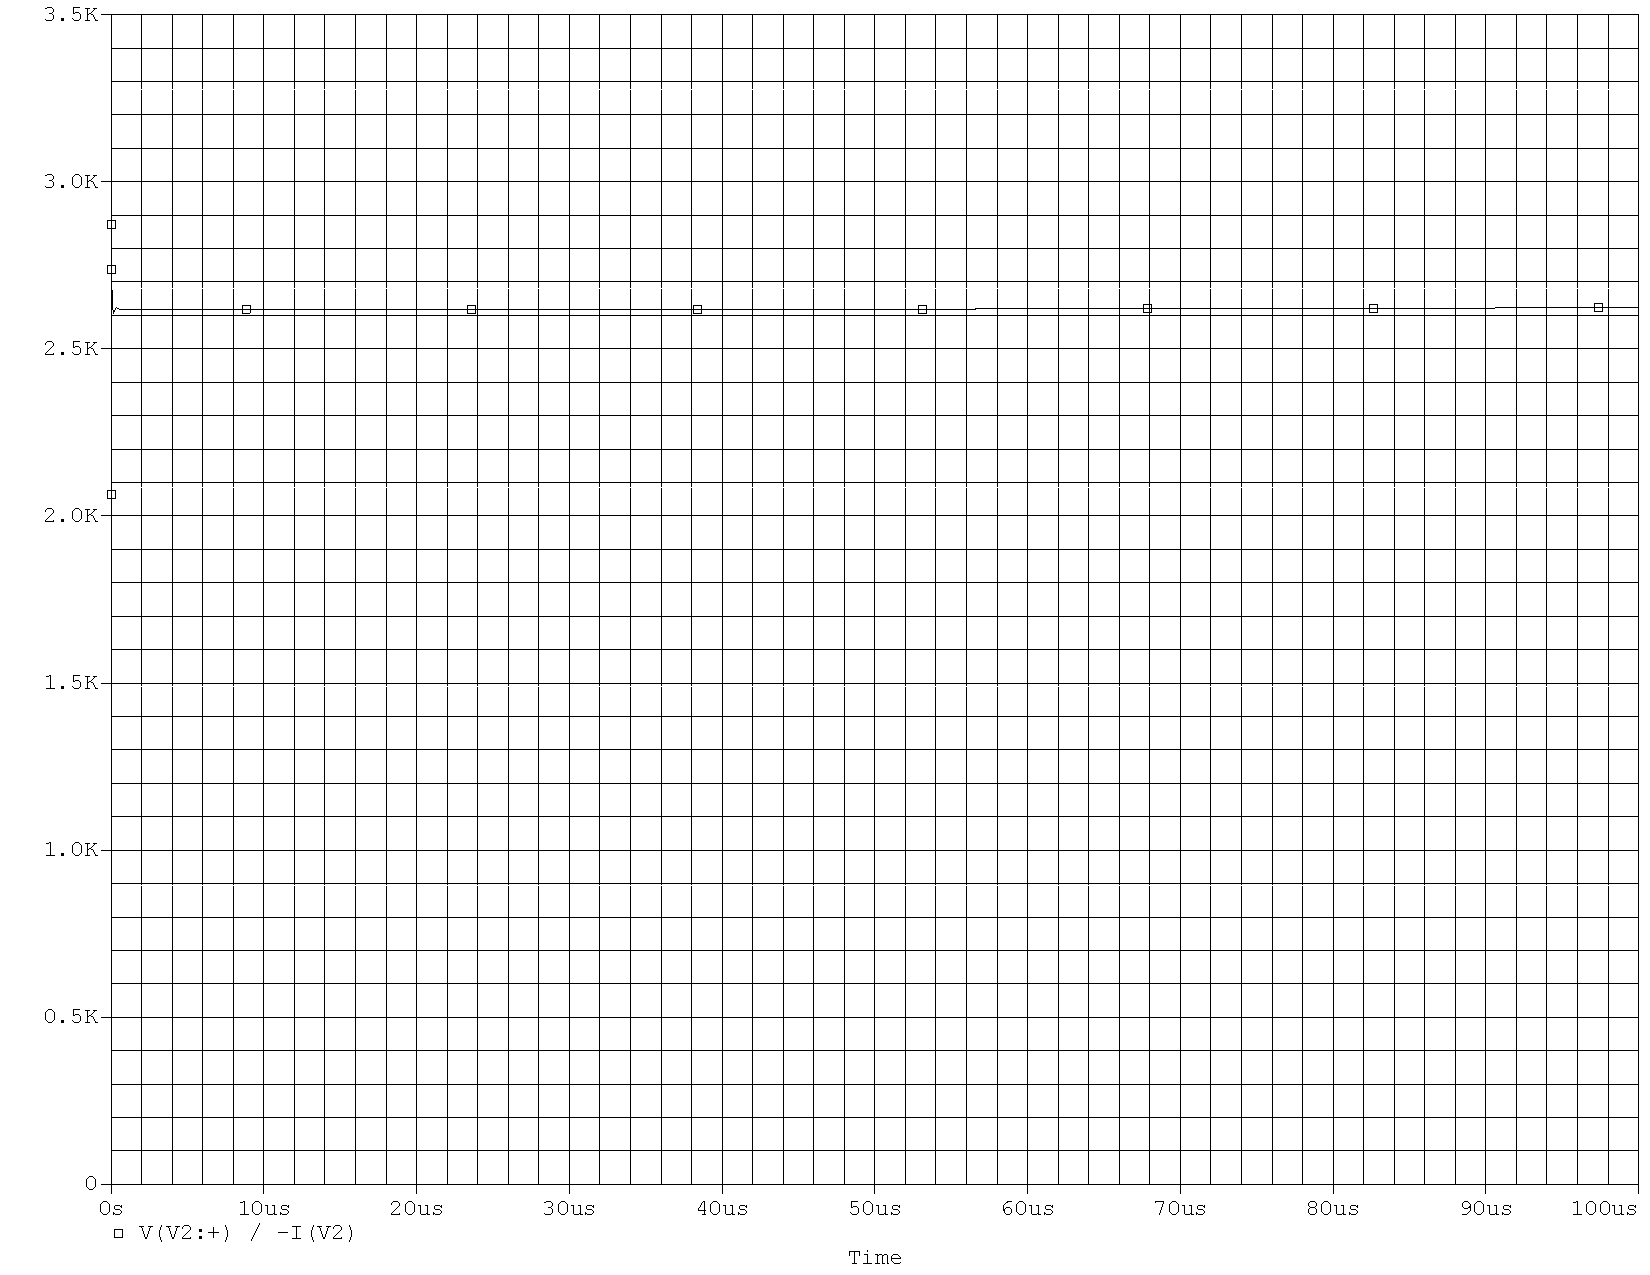
\includegraphics[width=\textwidth,height=\textheight,keepaspectratio]{Ulazna.pdf}
                \caption{Grafik za verifikaciju ulazne otpornosti}
                \label{Ulazna}
            \end{figure}
            \begin{figure}[H]
                \centering
                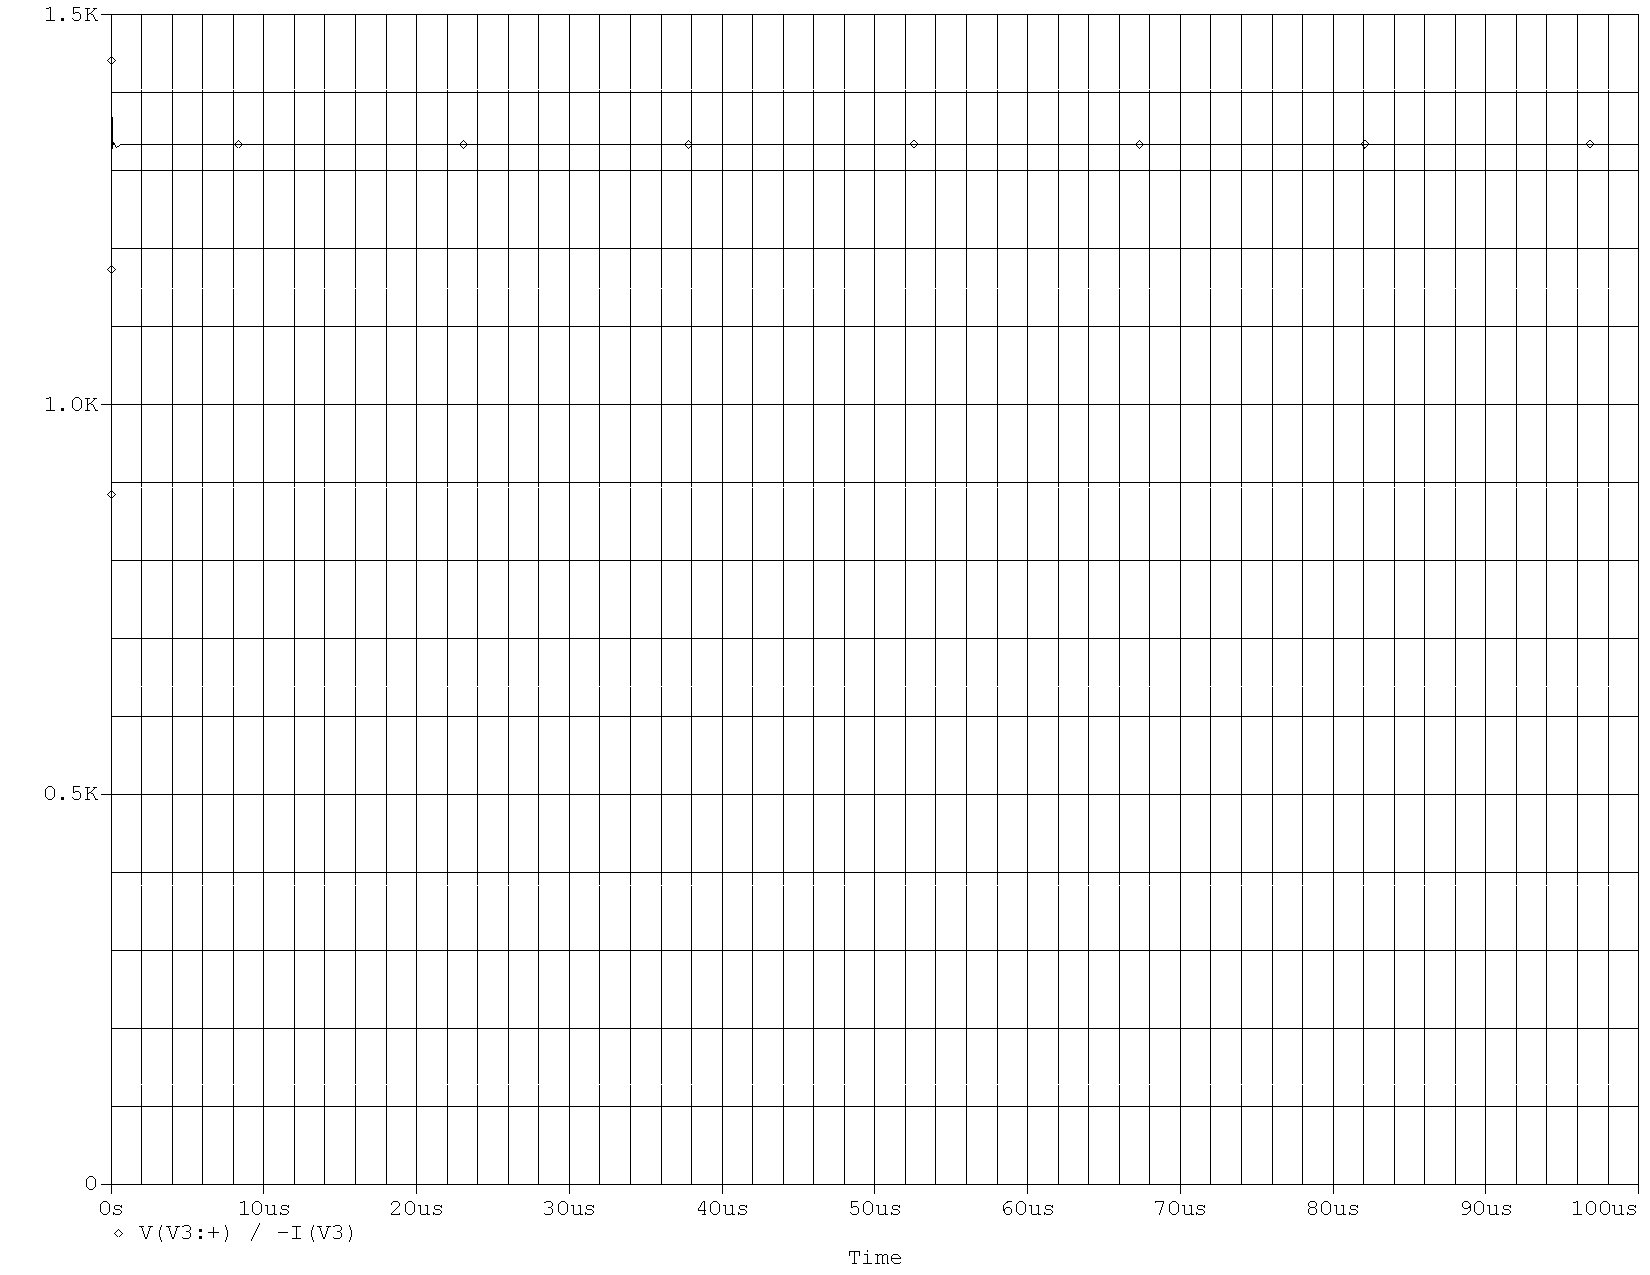
\includegraphics[width=\textwidth,height=\textheight,keepaspectratio]{Izlazna.pdf}
                \caption{Grafik za verifikaciju izlazne otpornosti}
                \label{Izlazna}
            \end{figure}
            \begin{figure}
                \centering
                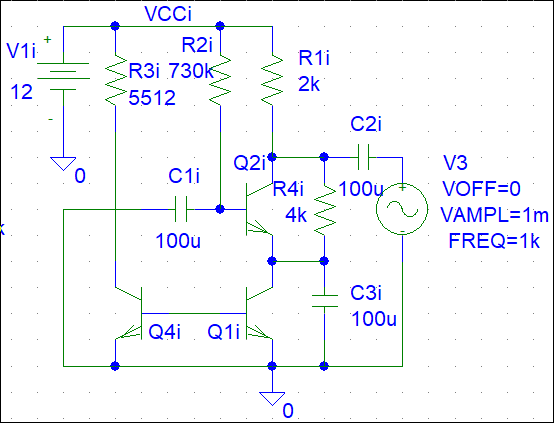
\includegraphics{CetvrtiKolo.png}
                \caption{Kolo za verifikaciju izlazne otpornosti}
                \label{CetvrtiKolo}
            \end{figure}
\end{document}
